% http://introlab.github.io/rtabmap/
\acs{rtabmap} is an open\hyp{}source \acs{rgbd}, stereo camera and, \acs{lidar} graph\hyp{}based \acs{slam} system. The system is based on an incremental appearence\hyp{}based loop closure detector. The detector uses a bag\hyp{}of\hyp{}words approach to determine how likely a new image comes from a previous or a new location. \acs{rtabmap} is a standalone application available for Ubuntu, Mac OS X, Windows, and a Raspberry Pi. But, also as a \acs{ros} package and on the Google Play Store. It is a heavily maintained piece of software. \cite{rtabmap_introlab}

The \acs{ros} package of \acs{rtabmap} has a lot of parameters to be adjusted to a specific need. The build\hyp{}in support with OctoMap allows it to be used for path planning. \acs{rtabmap} meets all the requirements needed for this project.

\begin{figure}[!h]
  \centering
  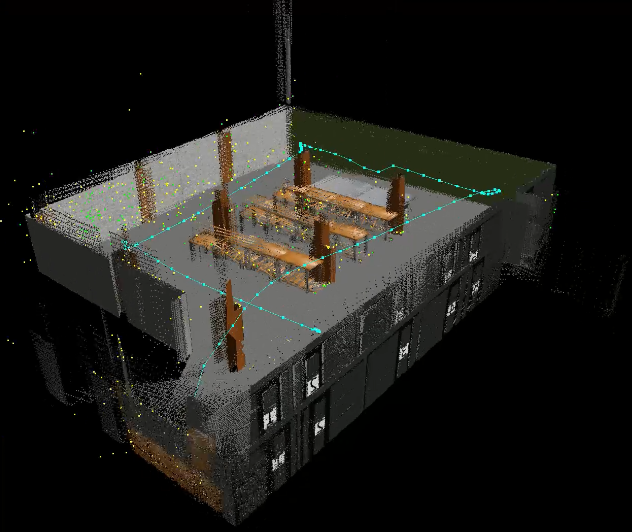
\includegraphics[width=0.7\linewidth]{rtabmap_implementation.png}
  \caption{Implementation of \acs{rtabmap}}
  \label{fig:rtabmap_implementation}
\end{figure}